\documentclass[12pt]{article}
\usepackage[margin=1in]{geometry}
\usepackage{amsmath,amsthm,amssymb}

% Ignore spaces in filenames
\usepackage[space]{grffile}

\usepackage[T1]{fontenc}
\usepackage{bigfoot} % to allow verbatim in footnote
\usepackage[numbered,framed]{matlab-prettifier}
\usepackage{filecontents}
\usepackage{graphicx}
\usepackage[normalem]{ulem}

\let\ph\mlplaceholder % shorter macro
\lstMakeShortInline"

\lstset{
  style              = Matlab-editor,
  basicstyle         = \mlttfamily,
  escapechar         = ",
  mlshowsectionrules = true,
}

\title{MAE 275 - Final}
\author{John Karasinski}
\date{June 10, 2015}

\begin{document}
\maketitle

\section{Defining the System}
The longitudinal linearized aircraft equations of motion can be expressed in state space form, with state variables $\Delta u, \Delta w, \Delta q, \Delta \theta, \Delta h$, as

\begin{equation*}
A =
\begin{bmatrix}
    X_u & X_w & 0 & -g \cos(\theta_0) & 0 \\
    \dfrac{Z_u}{1-Z_{\dot{w}}} & \dfrac{Z_w}{1-Z_{\dot{w}}} & \dfrac{Z_q + u_0}{1-Z_{\dot{w}}} & -\dfrac{g\sin \theta_0}{1-Z_{\dot{w}}} & 0 \\
    M_u + \dfrac{M_{\dot{w}} Z_u}{1-Z_{\dot{w}}} & M_w + \dfrac{M_{\dot{w}} Z_w}{1-Z_{\dot{w}}} & M_q + \dfrac{M_{\dot{w}} (Z_q + u_0)}{1-Z_{\dot{w}}} & -\dfrac{M_{\dot{w}} g\sin \theta_0}{1-Z_{\dot{w}}} & 0 \\
    0 & 0 & 1 & 0 & 0 \\
    0 & -1 & 0 & u_0 & 0
\end{bmatrix}
\end{equation*}

\noindent Relevant B, C, and D matrices can also be formed
\begin{equation*}
B =
\begin{bmatrix}
X_{\delta_e}                                                   & X_{\delta_T}                                                   & -X_u                                          & -X_w                                          & 0                                                    \\
\dfrac{Z_{\delta_e}}{1-Z_{\dot{w}}}                            & \dfrac{Z_{\delta_T}}{1-Z_{\dot{w}}}                            & \dfrac{-Z_u}{1-Z_{\dot{w}}}                   & \dfrac{-Z_w}{1-Z_{\dot{w}}}                   & \dfrac{-Z_q}{1-Z_{\dot{w}}}                          \\
M_{\delta_e} + \dfrac{M_{\dot{w}} Z_{\delta_e}}{1-Z_{\dot{w}}} & M_{\delta_T} + \dfrac{M_{\dot{w}} Z_{\delta_T}}{1-Z_{\dot{w}}} & -M_u - \dfrac{M_{\dot{w}} Z_u}{1-Z_{\dot{w}}} & -M_w - \dfrac{M_{\dot{w}} Z_w}{1-Z_{\dot{w}}} & -M_q -\dfrac{M_{\dot{w}} (Z_q + u_0)}{1-Z_{\dot{w}}} \\
    0   &  0   &  0   & 0 \\
    0   &  0   &  0   & 0 \\
\end{bmatrix}
\end{equation*}

$$
C =
\begin{bmatrix}
    1 & 0 & 0 & 0 & 0\\
    0 & 0 & 0 & 0 & 1\\
    0 & 0 & 0 & 1 & 0\\
\end{bmatrix},
\qquad
D =
\begin{bmatrix}
    0 & 0 & 0 & 0 & 0\\
    0 & 0 & 0 & 0 & 0\\
    0 & 0 & 0 & 0 & 0\\
\end{bmatrix}
$$

\clearpage
\noindent Plugging in the data for the A-7E aircraft in a landing approach to an aircraft carrier yields
\begin{equation*}
A =
\begin{bmatrix}
  -5.4534e-2 & +6.4327e-2 &          0 & -3.2200e+1 &           0 \\
  -2.8695e-1 & -5.2887e-1 & +2.1800e+2 &          0 &           0 \\
  -8.2071e-5 & -7.8112e-3 & -3.9053e-1 &          0 &           0 \\
           0 &          0 &          1 &          0 &           0 \\
           0 &         -1 &          0 & +2.1800e+2 &           0 \\
\end{bmatrix}
\end{equation*}

\begin{equation*}
B =
\begin{bmatrix}
  +7.3284e-1 & +1.3170e-3 & +5.4534e-2 & -6.4327e-2 &           0 \\
  -1.4714e+1 & -2.5000e-4 & +2.8695e-1 & +5.2887e-1 &           0 \\
  -2.1846e+0 & +4.0722e-6 & +8.2071e-5 & +7.8112e-3 & +3.9053e-01 \\
           0 &          0 &          0 &          0 &           0 \\
           0 &          0 &          0 &          0 &           0 \\
\end{bmatrix}
\end{equation*}

$$
C =
\begin{bmatrix}
    1 & 0 & 0 & 0 & 0\\
    0 & 0 & 0 & 0 & 1\\
    0 & 0 & 0 & 1 & 0\\
\end{bmatrix},
\qquad
D =
\begin{bmatrix}
    0 & 0 & 0 & 0 & 0\\
    0 & 0 & 0 & 0 & 0\\
    0 & 0 & 0 & 0 & 0\\
\end{bmatrix}
$$

\clearpage
\section{Handling Qualities}
The handling qualities of the pitch-rate SCAS can be estimated using the Bandwidth/Phase-Delay boundaries explained in the handout. The bandwidth is defined as the lesser of $w_{BW_{gain}}$ and $w_{BW_{phase}}$, which is 3.09 rad/s. The phase delay, $\tau_p$ is defined
\begin{equation*}
\tau_p = \dfrac{\Delta \Phi 2w_{180}}{57.3 (2w_{180})} = \dfrac{244-180}{57.3 (12.8)} = 0.09 \mbox{s}
\end{equation*}
These values suggest Level 1 handling qualities.
\begin{figure}[h!]
\begin{center}
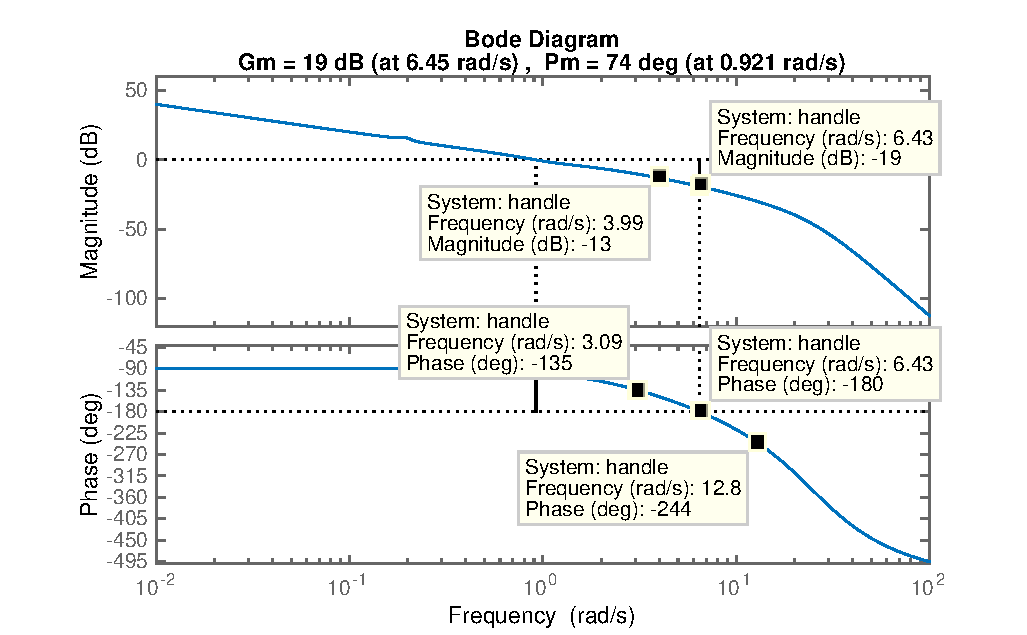
\includegraphics[height=.4\textheight]{figures/handling}
\caption{Closed-loop Bode with relevant points selected}
\end{center}
\end{figure}

\begin{figure}[h!]
\begin{center}
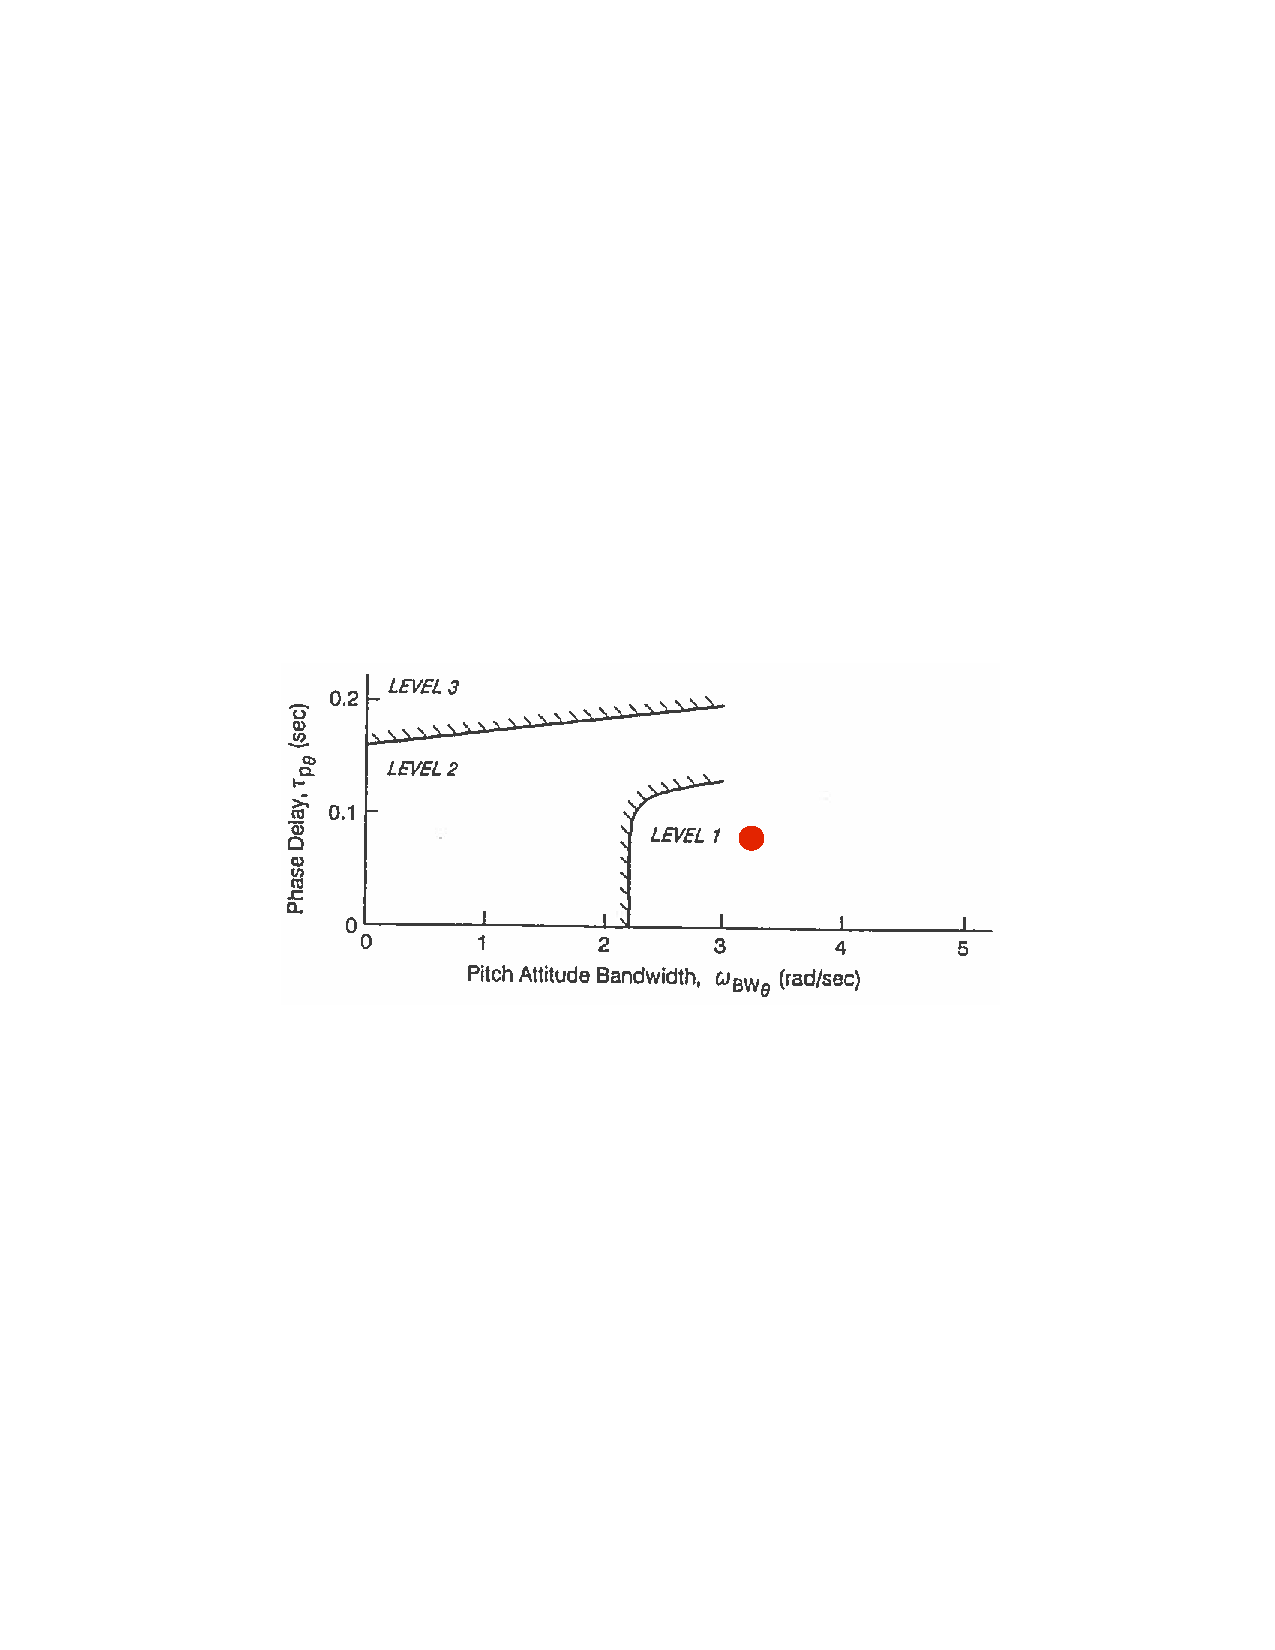
\includegraphics[height=.2\textheight]{figures/handling_marked}
\caption{Handling qualities plot with location marked}
\end{center}
\end{figure}

\end{document}
